\section{Running the QSM Emulator}\label{appsec:runningemulator}
\begin{quote}
Note: Figures in this section are from an earlier version of the
emulator
and will be updated as some point in time. The general instructions on
how to run the emulator are still applicable.
\end{quote}
\subsection{Window layout}
When starting the simulator with the command \texttt{emlqpl},
The first thing seen is \ref{fig:emulator}

\begin{figure}[htbp]
\centering
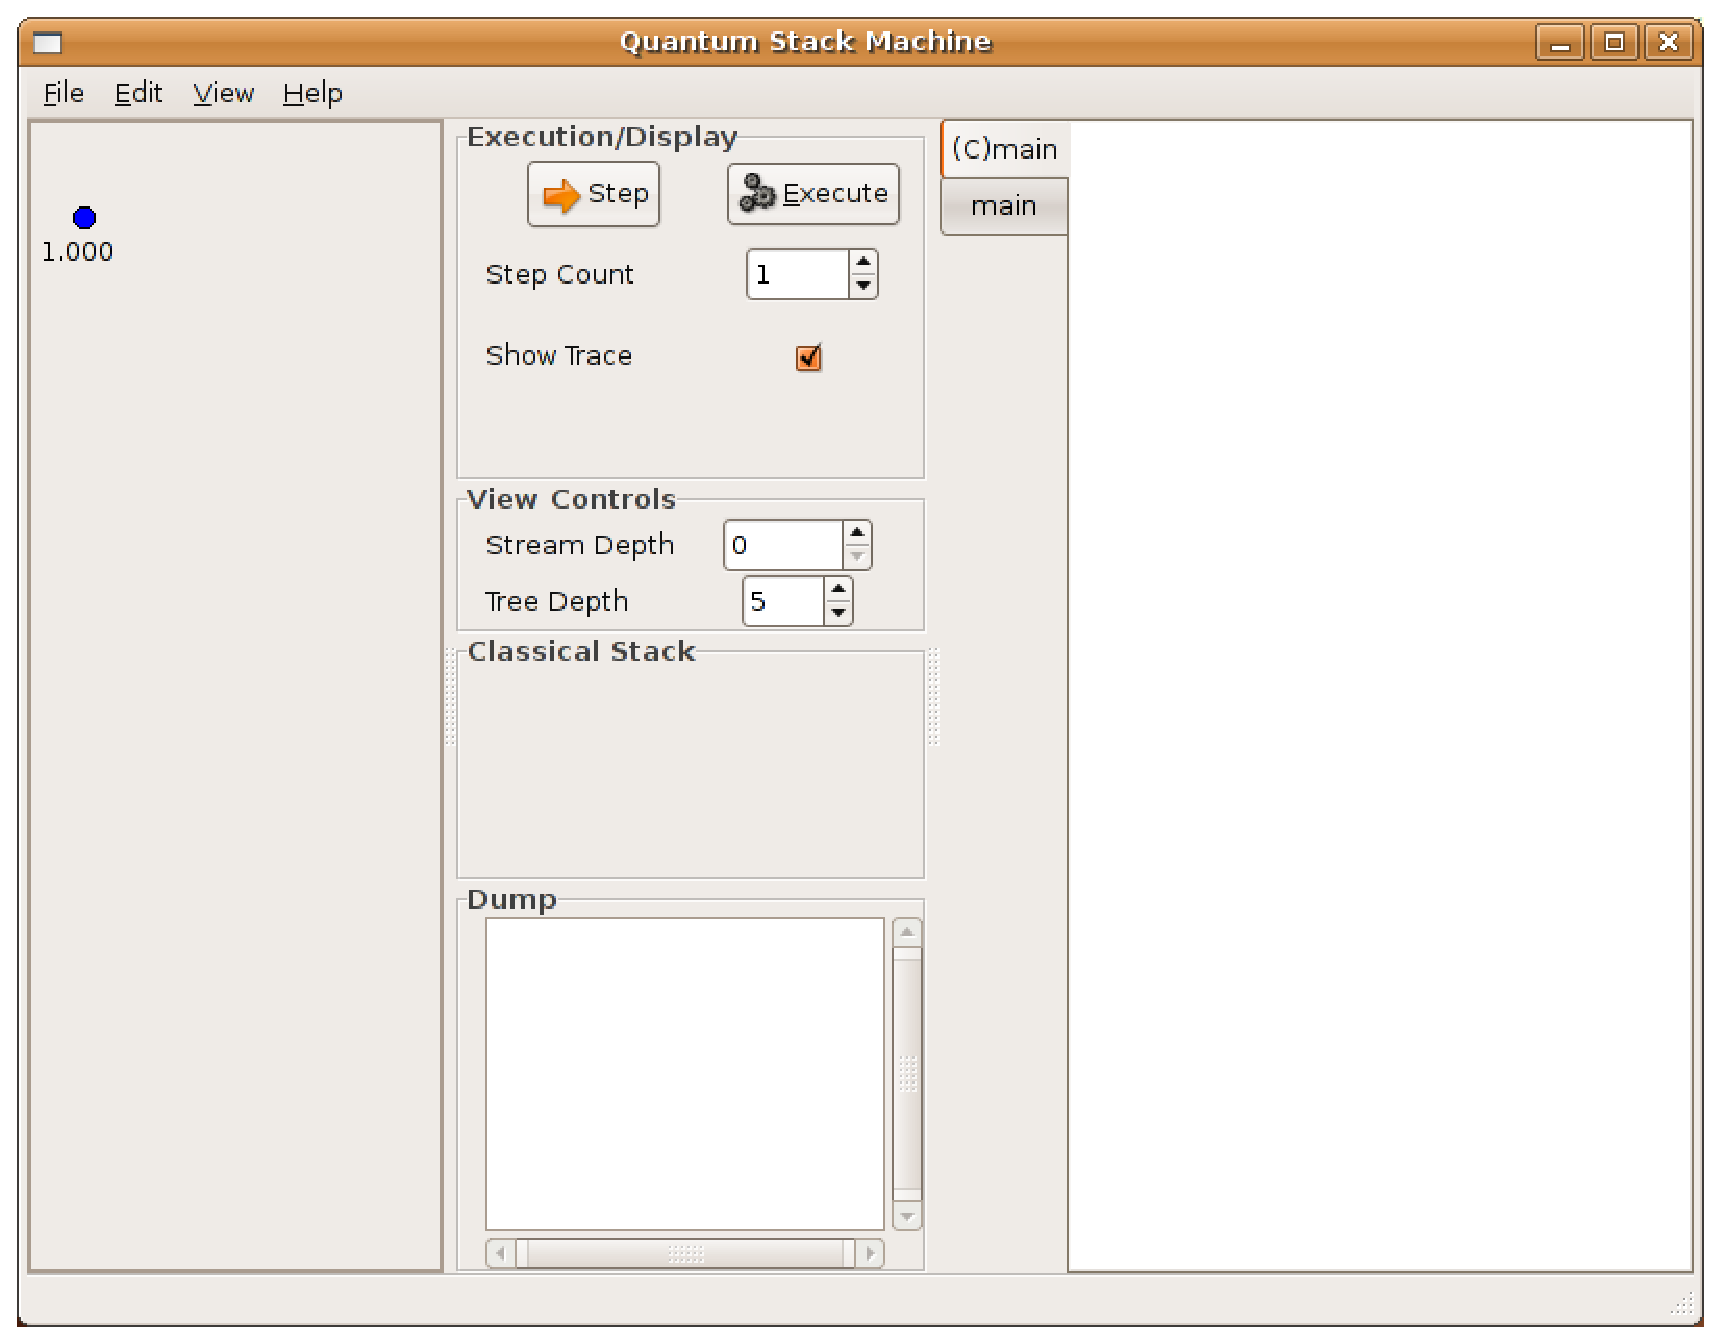
\includegraphics[scale=.5]{images/emulator/EmulatorAtStart.eps}
\caption{The emulator window}\label{fig:emulator}
\end{figure}

The emulator window is composed of three main sections. On the left is
the quantum stack display area. On the right is a tabbed display of the 
emulator assembly/machine code.
 
The middle section is divided into four parts. At the top is 
an execution and display control area followed by a view control area.
Beneath these is the  classical stack display area with
 the dump display area at the bottom.

\subsection{Loading a file}
The first required step is to actually load a program into the emulator,
using the \visctrl{File ---> Open} dialog in \ref{fig:emfileopen}.

\begin{figure}[htbp]
\centering
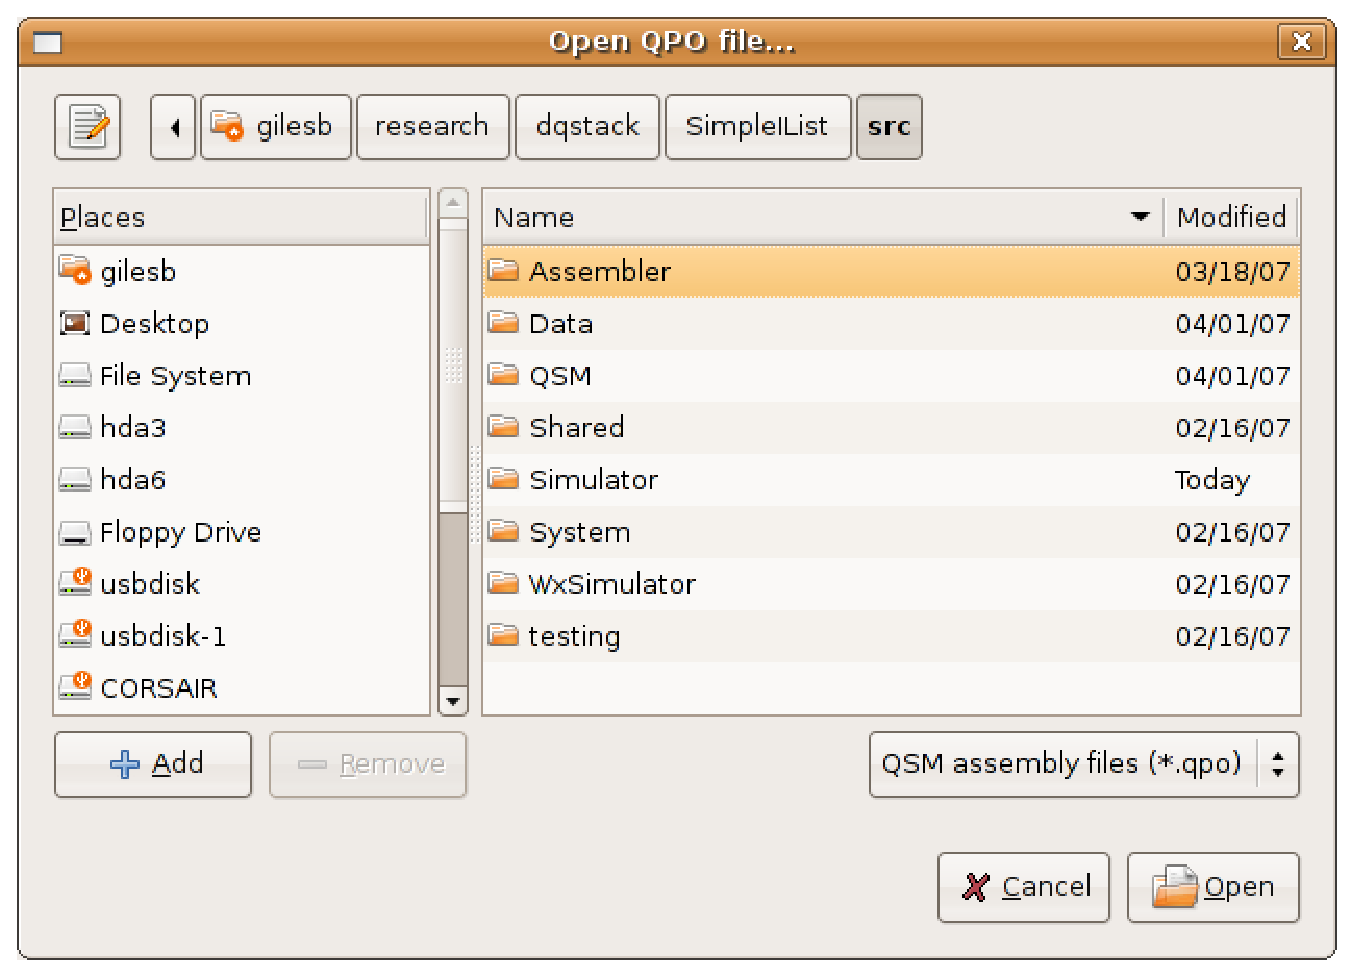
\includegraphics[scale=.5]{images/emulator/OpenDialog.eps}
\caption{Emulator file open dialog}\label{fig:emfileopen}
\end{figure}

Opening a QSM assembly file will check the compiler version 
used to create it and translate it to machine code. If the compiler and
emulator versions do not match, a warning dialog, as 
in \ref{fig:emversionmismatch} will appear. It is suggested that one 
ensures the version of the compiler and emulator are the same. 

\begin{figure}[htbp]
\centering
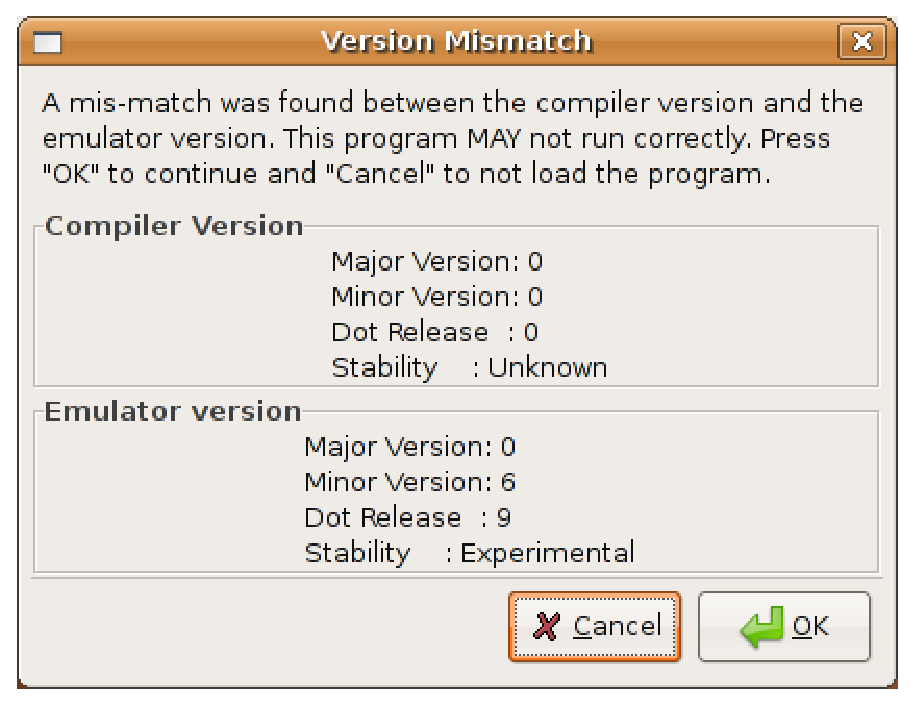
\includegraphics[scale=.5]{images/emulator/VersionMismatch.eps}
\caption{Version mis-match warning}\label{fig:emversionmismatch}
\end{figure}

After a successful assemble, the assembled code will appear in the right 
hand side. In a program, each function will appear as a separate tab in the
tabbed code window. The currently executing code will be in the top tab,
which is labelled with a ``(C)'' and the name of the currently executing 
function. Clicking on a tab will show the code associated with that tab.

\subsection{Setting preferences}

\begin{figure}[htbp]
\centering
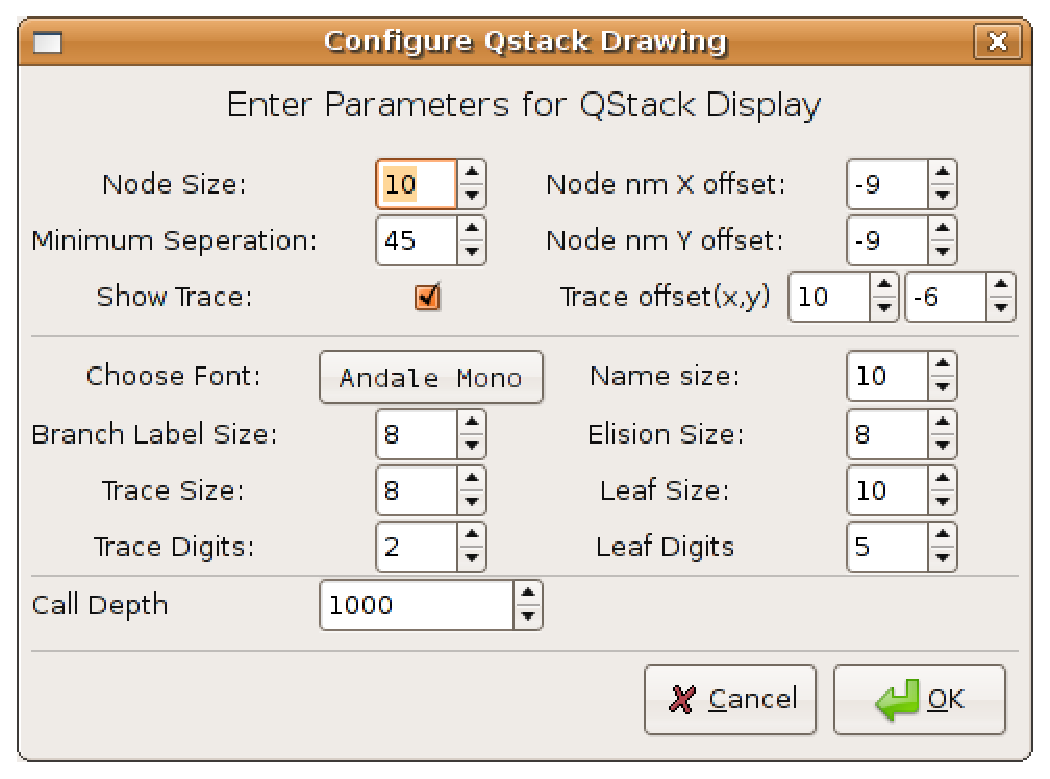
\includegraphics[scale=.5]{images/emulator/ConfigureQstackDisplay.eps}
\caption{Preferences dialog}\label{fig:emconfigure}
\end{figure}

Prior to executing the program, various display and execution options may
be set by using the \visctrl{Edit ---> Preferences} dialog, shown in 
\ref{fig:emconfigure}. The top third of the dialog controls the spacing and
size of nodes and their labels. The middle controls the font used and the 
font size choices for various labels.  Typically, the defaults for these
are sufficient for general execution.  

The final section, with the single item \visctrl{Call Depth} is used
to control the actual depth of recursion \emph{multiplied by the depth in
the stream.} In \ref{fig:emconfigure} the call depth is $1000$, meaning
that at stream depth 0, we will perform 1000 calls before 
signalling non-termination, at stream depth 5, 6000 calls and so on.

\subsection{Running the program}

\begin{figure}[htbp]
\centering
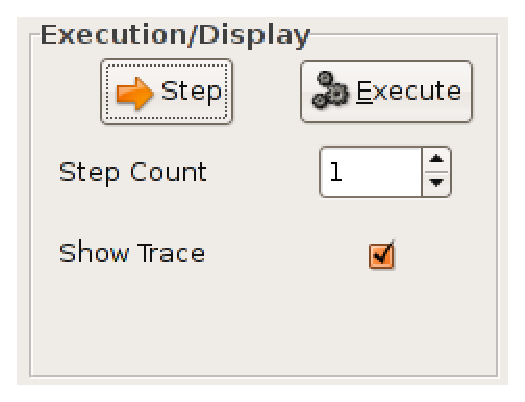
\includegraphics[scale=.8]{images/emulator/ExecutionDisplay.eps}
\caption{Execution control section of the main window}\label{fig:emexecdisplay}
\end{figure}

The program execution is controlled by the elements of the 
\visctrl{Execution/Display} section of the main window. As shown in 
\ref{fig:emexecdisplay}, there are two buttons (\visctrl{Step} and
\visctrl{Execute}), a spin control (\visctrl{Step Count}) and a 
checkbox (\visctrl{Show Trace}).

For each click of the \visctrl{Step} button, the emulator will execute
\emph{\visctrl{Step Count}} instructions and then redisplay the 
components of the quantum stack machine. The spin control may be set to 
any positive number.

The \visctrl{Execute} button will run the program until it completes. 
Completion may either be due to non-termination (e.g., exceeding the call
depth number of calls at the current stream depth), or actual completion.
See the  description of \visctrl{Stream Depth} below.
As well, while executing, the program will display a progress bar below the
\visctrl{Show Trace} area.  After completion, the machine components will
be re-displayed.

\begin{figure}[htbp]
\centering
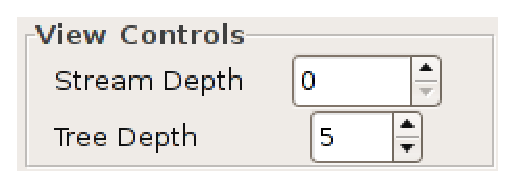
\includegraphics[scale=.8]{images/emulator/ViewControls.eps}
\caption{View controls section of the main window}\label{fig:emviewcontrols}
\end{figure}

The other component that affects execution in both  step mode and 
execute mode is the \visctrl{Stream Depth}, shown 
in \ref{fig:emviewcontrols}. Essentially, if one encounters a 
non-termination (a zero quantum stack) after executing, just increase the 
\visctrl{Stream Depth} and continue.

\subsection{Result interpretation}
Obviously, the first step is to visually examine the quantum stack. In case
where a simple final result is produced, this is often enough.

However, in cases where there are a significant number of nodes with multiple
branches, it can be difficult to determine what the results actually are.

\begin{figure}[htbp]
\centering
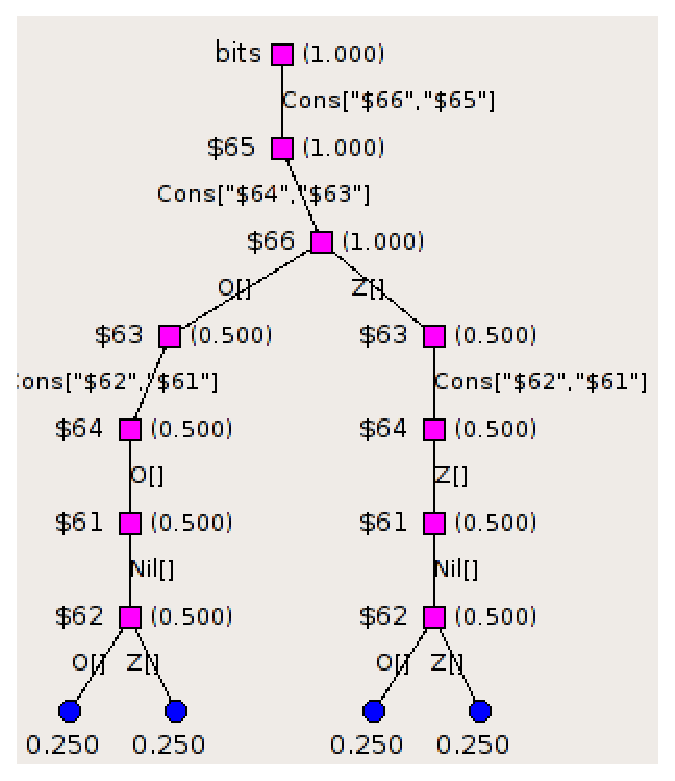
\includegraphics[scale=.75]{images/emulator/SimonsResult.eps}
\caption{Quantum stack at end of Simon's algorithm}\label{fig:emsimonsresult}
\end{figure}

For example, consider the end result of running Simon's algorithm, as shown
in \ref{fig:emsimonsresult}. The important result is ``What are the 
resulting bit-strings?''\footnote{Obviously, it is possible to determine 
the results solely by examination of the quantum stack as displayed. The 
method shown here becomes more relevant the more complicated the 
result stack.}. Using the menu item \visctrl{File ---> Simulate}, we
bring up a simulation dialog, which does the ``roll the dice'' and 
shows us what our end result would be when transferred to a classical
computer. For example, for three invocation of simulation, we 
get sub-figures (a), (b), and (c) as shown in \ref{fig:emsimonsims}.

\begin{figure}[htbp]
\centering
\subfloat[First simulation]{
\includegraphics[scale=.7]{images/emulator/SimonsSimulate1.eps}
}
\subfloat[Second simulation]{
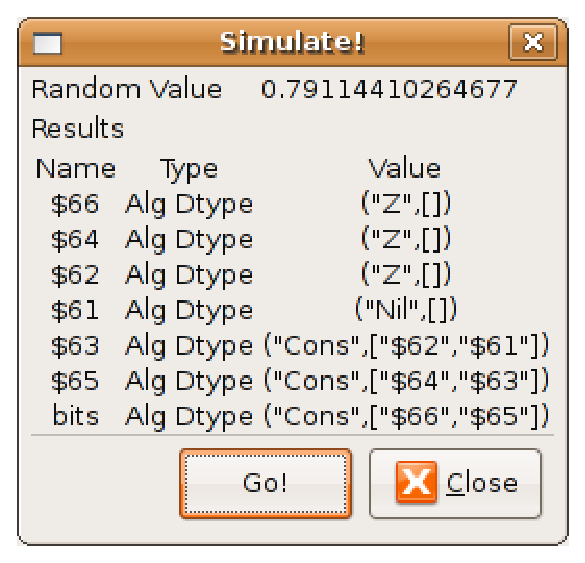
\includegraphics[scale=.7]{images/emulator/SimonsSimulate2.eps}
}
\subfloat[Third simulation]{
\includegraphics[scale=.7]{images/emulator/SimonsSimulate3.eps}
}
\caption{Simulation of  Simon's algorithm}\label{fig:emsimonsims}
\end{figure}

Note that the bit string can simply be read from the top three entries 
in the simulation results. It should also be noted that the additional
simulations do not require re-execution by the emulator. Instead, a new
random value is generated and used to determine a single path down the 
quantum stack for the values.




